\documentclass[11pt, a4paper, twoside, openright]{article}

% Algorithms
	%\usepackage{algpseudocode}
	%\usepackage{algorithm}

% Babel
\usepackage[english]{babel}

% Code writing
	%\usepackage[procnames]{listings}

% Font
\usepackage[utf8]{inputenc}
\usepackage[T1]{fontenc}
\usepackage{amssymb,amsmath,amsthm,amsfonts}
\usepackage{eucal}
\usepackage{textcomp}

% Footnote


% Hyperref
\usepackage[hyphens]{url}
\usepackage{cite}
\usepackage{hyperref}
\usepackage{nameref}
\usepackage{url}
% Images
\usepackage[pdftex]{graphicx}
	%\usepackage{subfigure}
\usepackage{subfig}
\usepackage{eso-pic}
\usepackage{caption}
\usepackage{wrapfig}
\usepackage{float}

% List
\usepackage{enumerate}

% SI units
\usepackage{siunitx}

% Standalone
\usepackage[subpreambles=true]{standalone}
\usepackage{import}

% Tables
\usepackage{tabularx}
\usepackage{booktabs}
\usepackage{multirow}

% TiKz and graphs
\usepackage{pgf,tikz,pgfplots}
% \usepackage{gnuplottex}
\usepackage{bm}
\usepackage{relsize}
%\usepackage[compat=1.1.0]{tikz-feynman}
\usepackage{circuitikz}

% Typeset
%\usepackage[top=2cm,bottom=2cm,left=2cm,right=2cm]{geometry}
\usepackage[top=2cm,bottom=2cm,left=2cm,right=2cm]{geometry}
\usepackage{fancyhdr}
\usepackage{indentfirst}
\usepackage{titlesec}
\usepackage{setspace}
\usepackage{xspace}
% \usepackage{parskip}  % Elimina il separatore a inizio paragrafo
\usepackage{afterpage}
\usepackage{comment}

%Python
\usepackage{xcolor}
\usepackage{listings}
\usepackage{framed}

%Per scrivere matrice identità
\usepackage{bbold}
%Per semplificazione formule
\usepackage{cancel}

%Evidenziare formule
\usepackage{empheq}
	%oppure
	%\usepackage{xcolor}
\usepackage{soul}

%Evidenziare testo con mdframed
\usepackage{mdframed}

%Note a margine
\usepackage{marginnote}

%Display data
\usepackage{datetime}

%Physics
\usepackage{physics}

%Geometry
%\newgeometry{inner=20mm,
%            outer=49mm,% = marginparsep + marginparwidth
%                       %   + 5mm (between marginpar and page border)
%            top=20mm,
%            bottom=25mm,
%            marginparsep=6mm,
%            marginparwidth=30mm}
%\makeatletter
%\renewcommand{\@marginparreset}{%
%  \reset@font\small
%  \raggedright
%  \slshape
%  \@setminipage
%}
%\makeatother

%Atom Latex
%\pgfplotsset{compat=1.15}

%%
\captionsetup[table]{font=small,labelfont={bf},skip=10pt}
\captionsetup[figure]{font=small,labelfont={bf},skip=10pt}

%intestazione pagina
%\pagestyle{fancy}
%\fancyhf{}
%\fancyhead[RE]{\ifnum\value{chapter}>0\nouppercase{\leftmark}\fi}
%\fancyhead[LE]{\small\textbf{\thepage}}
%\fancyhead[LO]{\nouppercase{\rightmark}}
%\fancyhead[RO]{\small\textbf{\thepage}}

%link ipertestuale per indice
\hypersetup{
	colorlinks=false,
	linkcolor=black,
	filecolor=blue,
	citecolor = blue,
	urlcolor=blue,
	}

%%%%%indent%%%
\setlength{\parindent}{15pt}
\setlength{\parskip}{0pt}


%boh
%\renewcommand{\chaptermark}[1]{%
% \markboth{\MakeUppercase{%
% \chaptername}\ \thechapter.%
% \ #1}{}}


 %Python in latex
 \definecolor{codegreen}{rgb}{0,0.6,0}
\definecolor{codegray}{rgb}{0.5,0.5,0.5}
\definecolor{codepurple}{rgb}{0.58,0,0.82}
\definecolor{backcolour}{rgb}{0.95,0.95,0.92}
\definecolor{commentcolour}{rgb}{0.43,0.63,0.65}

\definecolor{shadecolor}{rgb}{0.93, 0.93, 0.93}
\definecolor{darkgreen}{rgb}{0.0, 0.5, 0.0}
\definecolor{darkred}{rgb}{0.8, 0.0, 0.0}
\definecolor{violet}{rgb}{0.55, 0.0, 0.55}

\lstdefinestyle{mystyle}{ %Stile python code
    backgroundcolor=\color{shadecolor},
    commentstyle=\color{commentcolour},
    keywordstyle=\color{darkgreen},
    numberstyle=\tiny\color{codegray},
    stringstyle=\color{darkred},
    basicstyle=\footnotesize\ttfamily,
    breakatwhitespace=false,
    breaklines=true,
    captionpos=b,
    keepspaces=true,
    numbers=left,
    numbersep=5pt,
    showspaces=false,
    showstringspaces=false,
    showtabs=false,
    tabsize=2
}

\lstset{
    style=mystyle
}

%VHDL in latex
\usepackage{beramono}
\lstdefinelanguage{VHDL}{
   morekeywords={
     library,use,all,entity,is,port,in,out,end,architecture,of,
     begin,and
   },
   morecomment=[l]--
}
\colorlet{keyword}{blue!100!black!80}
\colorlet{comment}{green!90!black!90}
\lstdefinestyle{vhdl}{
   language     = VHDL,
   basicstyle   = \ttfamily\footnotesize,
   keywordstyle = \color{keyword}\bfseries,
   commentstyle = \color{comment}
}


% Derivatives
\renewcommand{\d}[0]{\mathrm{d}}
\newcommand{\dev}[2]{\displaystyle \frac{\d #1}{\d #2}}
\newcommand{\pdev}[2]{\displaystyle \frac{\partial #1}{\partial #2}}
\newcommand{\ndev}[3]{\displaystyle \frac{\d^{#3} #1}{\d #2^{#3} } }
\newcommand{\npdev}[3]{\displaystyle \frac{\partial^{#3} #1}{\partial #2^{#3} } }


%% Norms
\newcommand{\absvec}[1]{| \vec{#1} |}
\newcommand{\normvec}[1]{|\!| \vec{#1} |\!|}

\newcommand{\vmed}[1]{\left \langle #1 \right \rangle}
\newcommand{\vmedvec}[1]{\langle #1 \rangle}
\newcommand{\R}[0]{\mathbb{R}}
\renewcommand{\H}[0]{\operatorname{H}}

%Evidenziare formule
\newcommand{\mathcolorbox}[2]{\colorbox{#1}{$\displaystyle #2$}}
\newcommand{\hlfancy}[2]{\sethlcolor{#1}\hl{#2}}

%Theorem
\newtheorem{theorem}{Theorem}[section]
\newtheorem{corollary}{Corollary}[theorem]
\newtheorem{lemma}[theorem]{Lemma}
\newtheorem{proposition}[theorem]{Proposition}

\theoremstyle{definition}
\newtheorem{definition}{Definition}%[section]


%%%%%%%%%%%%%%%%%%%%Exercise and example%%%%%%%%%%%%%%%%%
\usepackage[many,most,theorems]{tcolorbox}


\newtcbtheorem{exercise}{Exercise}{ % frame stuff
    boxrule = 1pt,
    breakable,
    enhanced,
    frame empty,
    interior style= {blue!6},
    %interior empty,
    colframe=black,
    borderline ={1pt}{0pt}{black},
    left=0.2cm,
    % title stuff
    attach boxed title to top left={yshift=-2mm,xshift=0mm},
    coltitle=black,
    fonttitle=\bfseries,
    colbacktitle=white,
    boxed title style={boxrule=1pt,sharp corners}}{exercise} 

\newtcbtheorem{example}{Example}{ % frame stuff
    boxrule = 1pt,
    enhanced,
    frame empty,
    interior style= {green!6},%{left color=yellow!70,right color=green!70},
    %interior empty,
    colframe=black,
    borderline ={1pt}{0pt}{black},
    breakable,
    left=0.2cm,
    % title stuff
    attach boxed title to top left={yshift=-2mm,xshift=0mm},
    coltitle=black,
    fonttitle=\bfseries,
    colbacktitle=white,
    boxed title style={boxrule=1pt,sharp corners}}{example}
  
%\newtheorem{exercise}{Exercise}
%\newtheorem{example}{Example}

%%%%%%%%%%%%%%%%%%%%%%%%%%%%%%%%%%%

\theoremstyle{remark}
\newtheorem*{remark}{Remark}
\newtheorem{observation}{Observation}
%Evidenziare testo
\newtheorem*{solution}{Solution}

\newcommand\mybox[1]{%
  \fbox{\begin{minipage}{0.9\textwidth}#1\end{minipage}}}

  %Spiegazioni/verifiche
\newenvironment{greenbox}{\begin{mdframed}[hidealllines=true,backgroundcolor=green!20,innerleftmargin=3pt,innerrightmargin=3pt,innertopmargin=3pt,innerbottommargin=3pt]}{\end{mdframed}}

\newenvironment{bluebox}{\begin{mdframed}[hidealllines=true,backgroundcolor=blue!10,innerleftmargin=3pt,innerrightmargin=3pt,innertopmargin=3pt,innerbottommargin=3pt]}{\end{mdframed}}

\newenvironment{yellowbox}{\begin{mdframed}[hidealllines=true,backgroundcolor=yellow!20,innerleftmargin=3pt,innerrightmargin=3pt,innertopmargin=3pt,innerbottommargin=3pt]}{\end{mdframed}}

\newenvironment{redbox}{\begin{mdframed}[hidealllines=true,backgroundcolor=red!20,innerleftmargin=3pt,innerrightmargin=3pt,innertopmargin=3pt,innerbottommargin=3pt]}{\end{mdframed}}

\newenvironment{orangebox}{\begin{mdframed}[hidealllines=true,backgroundcolor=orange!20,innerleftmargin=3pt,innerrightmargin=3pt,innertopmargin=3pt,innerbottommargin=3pt]}{\end{mdframed}}

%emph equation
\newcommand*\myyellowbox[1]{%
  \colorbox{yellow!40}{\hspace{1em}#1\hspace{1em}}}

\newcommand*\mygreenbox[1]{%
  \colorbox{green!20}{\hspace{1em}#1\hspace{1em}}}
  
  
  
  
  

\usepackage{enumitem}

\begin{document}

\title{\textbf{Homework 3}}

\author{Alice Pagano \\ 1236916}

\maketitle

\section*{Second-order Feynman diagrams for the Green’s function}
\begin{enumerate}
\item  write the analytic expressions associated with diagrams (\textbf{a}), (\textbf{b}), and (\textbf{c}) in coordinate space;
\item show that (\textbf{c}) and (\textbf{d}) are distinct diagrams;
\item write the analytic expressions associated with diagram (\textbf{c}) in momentum space.
\end{enumerate}



\begin{figure}[h!]
\centering
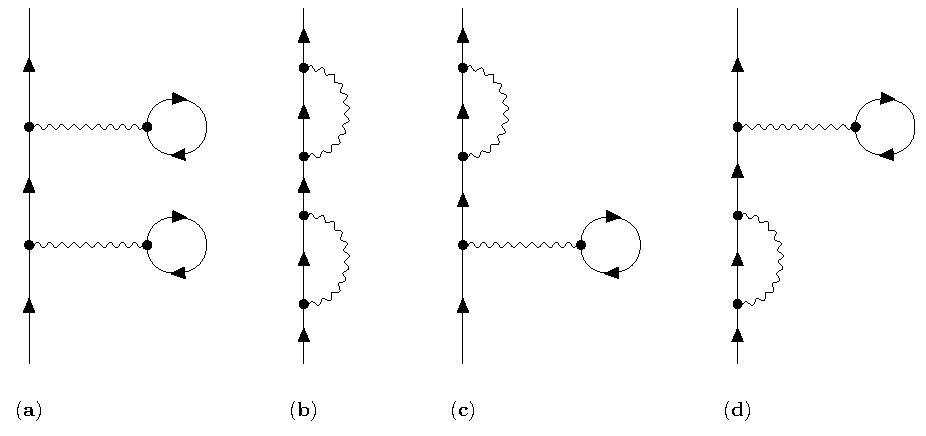
\includegraphics[width=0.9\textwidth]{images/tutti.pdf}
\caption{\label{fig:1} Four of the 10 topologically distinct connected diagrams at \( 2 \)-nd order perturbative expansion for the Green's function \( G_{\alpha \beta } (x,y) \).}
\end{figure}

%This is a good point to propose the third homework, which is related to the application of the feymann rules to build the different contribution to the green0s function. We focus on the second order ferymann diagrams. We have already shown them and the first four are these ones. We are invited to write the analityc expression using the feymann rules which are associated with the first three (a,b,c) diagrams (you have to write integrals with also spin label and so on ) in coordinate space. Then, considering that actually
%(c) and (d) diagrams look quite similar, just try to demonstrate that they are really topological distinct diagrams. Finally, just focus on (c) diagram and try to write the analytic expression of (c) diagram, also in momentum space and of course you can either use the feymann rules in momentum space or just take the fourier transform of the (c) contribution in coordinate space.

\section*{Solution}

\subsection*{1}
Let us write the analytic expression associated with diagrams (\textbf{a}), (\textbf{b}), and (\textbf{c}) in coordinate space, using the following \textbf{Feynman rules};
to find the \( n \)-th order contribution to the single-particle Green's function \( G_{\alpha \beta } (x,y) \) (for a system of identical particles interacting trough a 2-body potential):
\begin{enumerate}
\item Draw all topological distinct connected diagrams with \( n \) interaction lines \( U \) and \( (2n+1) \) fermion lines which correspond to the non-interacting Green's functions \( G^0 \).
\item Label each vertex with a four-dimensional space-time point \( x_i \).
\item Each solid line represents a Green's function \( G_{\alpha \beta }^0 (x,y) \) running from \( y \) to \( x \).
\item Each wavy line represents an interaction
\begin{equation*}
  U(x,x') = V(\va{x},\va{x}') \delta (t_x-t_{x'})
\end{equation*}
which is an instantaneous 2-body potential.
\item Integrate over all (space,time) variables that are internal and sum over the corresponding spin variables.

\item Affix a sign factor \( (-1)^F \) to each term, where \( F \) is the number of closed fermion loops in the diagram.

\item To compute \( G_{\alpha \beta }(x,y) \) assign a factor \( (i/\hbar )^n \) to each \( n \)-th order term.
\end{enumerate}

The diagrams in Fig.\ref{fig:1} are four of the 10 topologically distinct connected diagrams at the \( 2 \)-th order perturbative expansion for the Green's function \( G_{\alpha \beta } (x,y) \). Let us write the analityc expression of each of them:

\begin{enumerate}[label=(\alph*)]
\item For the first diagram, we obtain:

\begin{minipage}[]{0.35\linewidth}
\centering
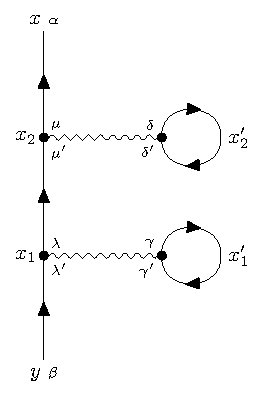
\includegraphics[width=0.9\textwidth]{images/A_label_c.pdf}
\label{}
\end{minipage}
\begin{minipage}[c]{0.65\linewidth}
\begin{equation}
\begin{split}
  G_{\alpha \beta }^{(2a)} (x,y) &= (-1)^2 \qty(\frac{i}{\hbar })^2
   \sum_{\substack{\lambda \lambda', \mu \mu' \\ \gamma \gamma', \delta \delta'   } }^{} \int_{}^{} \dd[4]{x_1} \int_{}^{} \dd[4]{x_1'} \int_{}^{} \dd[4]{x_2} \int_{}^{} \dd[4]{x_2'} \times \\
  & \times G_{\alpha \mu }^0 (x,x_2) U(x_2,x_2')_{\substack{ \mu \mu' \\ \delta \delta'} } G^0_{\mu' \lambda } (x_2,x_1) G^0_{\delta' \delta } (x_2',x_2') \times \\
  & \times U(x_1,x_1')_{\substack{ \lambda \lambda' \\ \gamma \gamma'} }
  G^0_{\lambda' \beta } (x_1,y) G^0_{\gamma' \gamma } (x_1',x_1')
\end{split}
\end{equation}
\end{minipage}

\item For the second diagram, we obtain:

\begin{minipage}[]{0.35\linewidth}
\centering
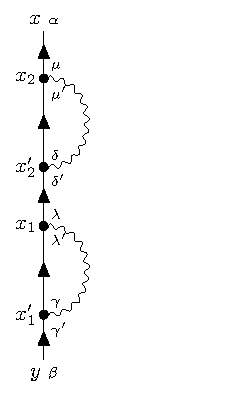
\includegraphics[width=0.9\textwidth]{images/B_label_c.pdf}
\label{}
\end{minipage}
\begin{minipage}[c]{0.65\linewidth}
\begin{equation}
\begin{split}
  G_{\alpha \beta }^{(2b)} (x,y) &= \qty(\frac{i}{\hbar })^2
   \sum_{\substack{\lambda \lambda', \mu \mu' \\ \gamma \gamma', \delta \delta'   } }^{} \int_{}^{} \dd[4]{x_1} \int_{}^{} \dd[4]{x_1'} \int_{}^{} \dd[4]{x_2} \int_{}^{} \dd[4]{x_2'} \times \\
  & \times G_{\alpha \mu }^0 (x,x_2) U(x_2,x_2')_{\substack{ \mu \mu' \\ \delta \delta'} } G^0_{\mu' \delta } (x_2,x_2') G^0_{\delta' \lambda } (x_2',x_1) \times \\
  & \times U(x_1,x_1')_{\substack{ \lambda \lambda' \\ \gamma \gamma'} }
  G^0_{\lambda' \gamma } (x_1,x_1') G^0_{\gamma' \beta } (x_1',y)
\end{split}
\end{equation}
\end{minipage}

\item For the third diagram, we obtain:

\begin{minipage}[]{0.35\linewidth}
\centering
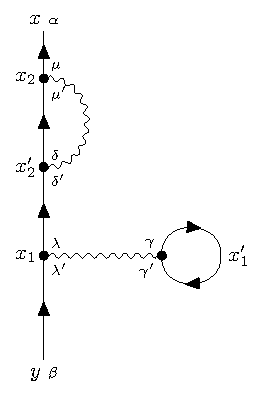
\includegraphics[width=0.9\textwidth]{images/C_label_c.pdf}
\label{}
\end{minipage}
\begin{minipage}[c]{0.65\linewidth}
\begin{equation}
\begin{split}
  G_{\alpha \beta }^{(2c)} (x,y) &= (-1)^1 \qty(\frac{i}{\hbar })^2
   \sum_{\substack{\lambda \lambda', \mu \mu' \\ \gamma \gamma', \delta \delta'   } }^{} \int_{}^{} \dd[4]{x_1} \int_{}^{} \dd[4]{x_1'} \int_{}^{} \dd[4]{x_2} \int_{}^{} \dd[4]{x_2'} \times \\
  & \times G_{\alpha \mu }^0 (x,x_2) U(x_2,x_2')_{\substack{ \mu \mu' \\ \delta \delta'} } G^0_{\mu' \delta } (x_2,x_2') G^0_{\delta' \lambda } (x_2',x_1) \times \\
  & \times U(x_1,x_1')_{\substack{ \lambda \lambda' \\ \gamma \gamma'} }
  G^0_{\lambda' \beta } (x_1,y) G^0_{\gamma' \gamma } (x_1',x_1')
\end{split}
\label{eq:c_analitic}
\end{equation}
\end{minipage}

\item For the fourth diagram, we obtain:

\begin{minipage}[]{0.35\linewidth}
\centering
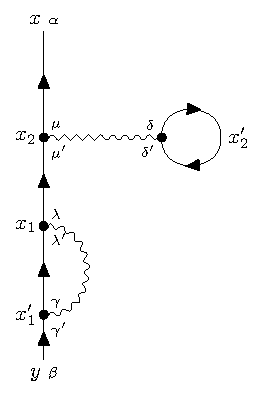
\includegraphics[width=0.9\textwidth]{images/D_label_c.pdf}
\label{}
\end{minipage}
\begin{minipage}[c]{0.65\linewidth}
\begin{equation}
\begin{split}
  G_{\alpha \beta }^{(2d)} (x,y) &= (-1)^1 \qty(\frac{i}{\hbar })^2
   \sum_{\substack{\lambda \lambda', \mu \mu' \\ \gamma \gamma', \delta \delta'   } }^{} \int_{}^{} \dd[4]{x_1} \int_{}^{} \dd[4]{x_1'} \int_{}^{} \dd[4]{x_2} \int_{}^{} \dd[4]{x_2'} \times \\
  & \times G_{\alpha \mu }^0 (x,x_2) U(x_2,x_2')_{\substack{ \mu \mu' \\ \delta \delta'} } G^0_{\mu' \lambda } (x_2,x_1) G^0_{\delta' \delta } (x_2',x_2') \times \\
  & \times U(x_1,x_1')_{\substack{ \lambda \lambda' \\ \gamma \gamma'} }
  G^0_{\lambda' \gamma } (x_1,x_1') G^0_{\gamma' \beta } (x_1',y)
\end{split}
\end{equation}
\end{minipage}

\end{enumerate}


\subsection*{2}
Let us note that with the Feynman method, the arrows designate the direction of momentum flow. It is because of the arrows that the diagrams (\textbf{c}) and (\textbf{d}) are topologically distinct.
In particular, graphically two diagrams are topologically distinct in the Feynman sense if they are visualized as made of rubber bands and one cannot be deformed into the other.


Now, in order to see analitically that diagram (\textbf{c}) and (\textbf{d}) are distinct, let us rewrite the analityc formula for the two diagrams by highliting their differences. For the (\textbf{c}) diagram:
\begin{equation*}
\begin{split}
  G_{\alpha \beta }^{(2c)} (x,y) &= (-1)^1 \qty(\frac{i}{\hbar })^2
   \sum_{\substack{\lambda \lambda', \mu \mu' \\ \gamma \gamma', \delta \delta'   } }^{} \int_{}^{} \dd[4]{x_1} \int_{}^{} \dd[4]{x_1'} \int_{}^{} \dd[4]{x_2} \int_{}^{} \dd[4]{x_2'}
   \times G_{\alpha \mu }^0 (x,x_2) U(x_2,x_2')_{\substack{ \mu \mu' \\ \delta \delta'} } \times \\
  & \times \mathcolorbox{green!20}{G^0_{\mu' \delta } (x_2,x_2')
  G^0_{\delta' \lambda } (x_2',x_1) }
  U(x_1,x_1')_{\substack{ \lambda \lambda' \\ \gamma \gamma'} }
  \mathcolorbox{green!20}{
  G^0_{\lambda' \beta } (x_1,y) G^0_{\gamma' \gamma } (x_1',x_1')
  }
\end{split}
\end{equation*}
while for the (\textbf{d}) diagram:
\begin{equation*}
\begin{split}
  G_{\alpha \beta }^{(2d)} (x,y) &= (-1)^1 \qty(\frac{i}{\hbar })^2
   \sum_{\substack{\lambda \lambda', \mu \mu' \\ \gamma \gamma', \delta \delta'   } }^{} \int_{}^{} \dd[4]{x_1} \int_{}^{} \dd[4]{x_1'} \int_{}^{} \dd[4]{x_2} \int_{}^{} \dd[4]{x_2'}
   G_{\alpha \mu }^0 (x,x_2) U(x_2,x_2')_{\substack{ \mu \mu' \\ \delta \delta'} } \times \\
  & \times \mathcolorbox{green!20}{G^0_{\mu' \lambda } (x_2,x_1) G^0_{\delta' \delta } (x_2',x_2') }
  U(x_1,x_1')_{\substack{ \lambda \lambda' \\ \gamma \gamma'} }
  \mathcolorbox{green!20}{
  G^0_{\lambda' \gamma } (x_1,x_1') G^0_{\gamma' \beta } (x_1',y)
  }
\end{split}
\end{equation*}
Let us see if with an exchange of the dummy variables, the two analityc formula are the same. For the internal variables we change in the following way:
\begin{equation*}
  x_1 \leftrightarrow  x_2, \quad  x_1' \leftrightarrow x_2'
\end{equation*}
while for the spin indices
\begin{equation*}
  \lambda  \leftrightarrow  \mu , \, \lambda' \leftrightarrow \mu', \,
  \gamma \leftrightarrow \delta, \gamma' \leftrightarrow \delta'
\end{equation*}
Now, we make these substitutions on the second equation (the analityc expression for the (\textbf{d}) diagram) obtaining:
\begin{equation*}
\begin{split}
  G_{\alpha \beta }^{(2d)} (x,y) &= (-1)^1 \qty(\frac{i}{\hbar })^2
   \sum_{\substack{\lambda \lambda', \mu \mu' \\ \gamma \gamma', \delta \delta'   } }^{} \int_{}^{} \dd[4]{x_2} \int_{}^{} \dd[4]{x_2'} \int_{}^{} \dd[4]{x_1} \int_{}^{} \dd[4]{x_1'}
   G_{\alpha \mu }^0 (x,x_1) U(x_1,x_1')_{\substack{ \mu \mu' \\ \delta \delta'} } \times \\
  & \times G^0_{\mu' \lambda } (x_1,x_2) G^0_{\delta' \delta } (x_1',x_1')
  U(x_2,x_2')_{\substack{ \lambda \lambda' \\ \gamma \gamma'} }
  G^0_{\lambda' \gamma } (x_2,x_2') G^0_{\gamma' \beta } (x_2',y)
\end{split}
\end{equation*}
we see that the result are still different. We cannot find any change of variables suitable.





\subsection*{3}
Finally, we just focus on (\textbf{c}) diagram and we write its analytic expression in momentum space either just taking the Fourier transform of its contribution in coordinate space and using the Feynman rules in momentum space.

\subsubsection*{Fourier antitransformation}
Let us consider the analitycal formula of the (\textbf{c}) diagram in coordinate space (Eq.\eqref{eq:c_analitic}):
\begin{equation*}
\begin{split}
  G_{\alpha \beta }^{(2c)} (x,y) &= (-1)^1 \qty(\frac{i}{\hbar })^2
   \sum_{\substack{\lambda \lambda', \mu \mu' \\ \gamma \gamma', \delta \delta'   } }^{} \int_{}^{} \dd[4]{x_1} \int_{}^{} \dd[4]{x_1'} \int_{}^{} \dd[4]{x_2} \int_{}^{} \dd[4]{x_2'}
  G_{\alpha \mu }^0 (x,x_2) U(x_2,x_2')_{\substack{ \mu \mu' \\ \delta \delta'} } \times \\
  & \times G^0_{\mu' \delta } (x_2,x_2') G^0_{\delta' \lambda } (x_2',x_1)
   U(x_1,x_1')_{\substack{ \lambda \lambda' \\ \gamma \gamma'} }
  G^0_{\lambda' \beta } (x_1,y) G^0_{\gamma' \gamma } (x_1',x_1')
\end{split}
\end{equation*}
If we suppose spatial and temporal invariance (\textbf{uniform system}) then we can write a full Fourier representation.
First of all, let us consider the Fourier transform of each term separately in the above expression:
\begin{subequations}
\begin{align*}
  U (x_2,x_2')_{\substack{ \mu \mu' \\ \delta \delta'} } &=  \frac{1}{(2 \pi )^4} \int_{}^{} \dd[4]{k_2} e^{i k_2 (x_2-x_2')} U (k_2)_{\substack{ \mu \mu' \\ \delta \delta'} } \\
  U (x_1,x_1')_{\substack{ \lambda \lambda' \\ \gamma \gamma'} } &=  \frac{1}{(2 \pi )^4} \int_{}^{} \dd[4]{k_1} e^{i k_1 (x_1-x_1')} U (k_1)_{\substack{ \lambda \lambda' \\ \gamma \gamma'} } \\
  G^0_{\alpha \mu } (x,x_2)&=  \frac{1}{(2 \pi )^4} \int_{}^{} \dd[4]{k} e^{i k (x-x_2)}   G^0_{\alpha \mu } (k) \\
  G^0_{\mu' \delta } (x_2,x_2') &=  \frac{1}{(2 \pi )^4} \int_{}^{} \dd[4]{q_1} e^{i q_1 (x_2-x_2')}   G^0_{\mu' \delta } (q_1) \\
  G^0_{\delta' \lambda } (x_2',x_1) &=  \frac{1}{(2 \pi )^4} \int_{}^{} \dd[4]{p_1} e^{i p_1 (x_2'-x_1)}   G^0_{\delta' \lambda  } (p_1) \\
  G^0_{\lambda' \beta } (x_1,y) &=  \frac{1}{(2 \pi )^4} \int_{}^{} \dd[4]{p_2} e^{i p_2 (x_1-y)}   G^0_{\lambda' \beta  } (p_2) \\
  G^0_{\gamma' \gamma } (x_1',x_1') &=  \frac{1}{(2 \pi )^4} \int_{}^{} \dd[4]{q_2} e^{i q_2 (x_1'-x_1')}   G^0_{\gamma' \gamma  } (q_2)
\end{align*}
\end{subequations}
By substituting the last expressions in the upper equation we obtain:
\begin{equation*}
\begin{split}
  G_{\alpha \beta }^{(2c)} (x,y) &= \frac{(-1)^1}{(2 \pi )^{28}} \qty(\frac{i}{\hbar })^2
   \sum_{\substack{\lambda \lambda', \mu \mu' \\ \gamma \gamma', \delta \delta'   } }^{} \int_{}^{} \dd[4]{x_1} \int_{}^{} \dd[4]{x_1'} \int_{}^{} \dd[4]{x_2} \int_{}^{} \dd[4]{x_2'} \int_{}^{} \dd[4]{k} \dd[4]{k_2} \dd[4]{q_1} \dd[4]{p_1} \dd[4]{k_1} \dd[4]{p_2} \dd[4]{q_2}  \times \\
   & \times G^0_{\alpha \mu } (k) U (k_2)_{\substack{ \mu \mu' \\ \delta \delta'} } G^0_{\mu' \delta } (q_1) G^0_{\delta' \lambda  } (p_1) U (k_1)_{\substack{ \lambda \lambda' \\ \gamma \gamma'} } G^0_{\lambda' \beta  } (p_2) G^0_{\gamma' \gamma  } (q_2) \times \\
   & \times e^{i k (x-x_2)} e^{i k_2 (x_2-x_2')} e^{i q_1 (x_2-x_2')} e^{i p_1 (x_2'-x_1)} e^{i k_1 (x_1-x_1')} e^{i p_2 (x_1-y)} \cancel{e^{i q_2 (x_1'-x_1')} }
\end{split}
\end{equation*}
If we consider the property:
\begin{equation*}
  \delta ^{(4)} (t) = \frac{1}{(2 \pi )^4} \int_{}^{} \dd[4]{x} e^{i t x}
\end{equation*}
we can integrate over the internal variables \( x_1,x_1',x_2,x_2' \) obtaining delta functions. Hence:
\begin{subequations}
\begin{align*}
  \int_{}^{} \dd[4]{x_2} e^{i (k_2+q_1-k)}   &= (2 \pi )^4 \delta ^{(4)} (k_2+q_1-k) \\
  \int_{}^{} \dd[4]{x_2'} e^{i (p_1-q_1-k_2)}   &= (2 \pi )^4 \delta ^{(4)} (p_1-q_1-k_2) \\
  \int_{}^{} \dd[4]{x_1} e^{i (k_1+p_2-p_1)}   &= (2 \pi )^4 \delta ^{(4)} (k_1+p_2-p_1) \\
  \int_{}^{} \dd[4]{x_1'} e^{i (-k_1)}   &= (2 \pi )^4 \delta ^{(4)} (-k_1) \\
\end{align*}
\end{subequations}
Thus the analitycal Fourier transformed expression for diagram (\textbf{c}) becomes:
\begin{equation*}
\begin{split}
  G_{\alpha \beta }^{(2c)} (x,y) &= \frac{(-1)^1}{(2 \pi )^{12}} \qty(\frac{i}{\hbar })^2
   \sum_{\substack{\lambda \lambda', \mu \mu' \\ \gamma \gamma', \delta \delta'   } }^{} \int_{}^{} \dd[4]{k} \dd[4]{k_2} \dd[4]{q_1} \dd[4]{p_1} \dd[4]{k_1} \dd[4]{p_2} \dd[4]{q_2}  \times \\
   & \times G^0_{\alpha \mu } (k) U (k_2)_{\substack{ \mu \mu' \\ \delta \delta'} } G^0_{\mu' \delta } (q_1) G^0_{\delta' \lambda  } (p_1) U (k_1)_{\substack{ \lambda \lambda' \\ \gamma \gamma'} } G^0_{\lambda' \beta  } (p_2) G^0_{\gamma' \gamma  } (q_2) \times \\
   & \times e^{i k x} e^{-i p_2 y }
   \delta ^{(4)} (k_2+q_1-k) \delta ^{(4)} (p_1-q_1-k_2) \delta ^{(4)} (k_1+p_2-p_1) \delta ^{(4)} (-k_1)
\end{split}
\end{equation*}
By exploiting the delta functions:
\begin{equation*}
  \begin{cases}
   k = k_2 + q_1 & \Rightarrow p_1 = k \\
   p_1 = q_1 + k_2 & \Rightarrow  k_2 = k - q_1 \\
   p_1 = k_1 + p_2 & \Rightarrow  p_2 = k \\
   -k_1 = 0 & \Rightarrow k_1=0
  \end{cases}
\end{equation*}
So, we can write:
\begin{equation*}
\begin{split}
  G_{\alpha \beta }^{(2c)} (x,y) &= \frac{(-1)^1}{(2 \pi )^{12}} \qty(\frac{i}{\hbar })^2
   \sum_{\substack{\lambda \lambda', \mu \mu' \\ \gamma \gamma', \delta \delta'   } }^{} \int_{}^{} \dd[4]{k} \int_{}^{} \dd[4]{q_1} \dd[4]{q_2}  e^{i k x} e^{-i k y } \times \\
   &
   \times G^0_{\alpha \mu } (k) U (k-q_1)_{\substack{ \mu \mu' \\ \delta \delta'} } G^0_{\mu' \delta } (q_1) G^0_{\delta' \lambda  } (k) U (0)_{\substack{ \lambda \lambda' \\ \gamma \gamma'} } G^0_{\lambda' \beta  } (k) G^0_{\gamma' \gamma  } (q_2)
\end{split}
\end{equation*}
More explicitly:
\begin{equation*}
\begin{split}
  G_{\alpha \beta }^{(2c)} (x,y) &= \frac{1}{(2 \pi )^4} \int_{}^{} \dd[4]{k} e^{i k (x-y)}
  \Big[ \frac{(-1)^1}{(2 \pi )^{8}} \qty(\frac{i}{\hbar })^2
   \sum_{\substack{\lambda \lambda', \mu \mu' \\ \gamma \gamma', \delta \delta'   } }^{}  \int_{}^{} \dd[4]{q_1} \dd[4]{q_2}   \times \\
   &
   \times G^0_{\alpha \mu } (k) U (k-q_1)_{\substack{ \mu \mu' \\ \delta \delta'} } G^0_{\mu' \delta } (q_1) G^0_{\delta' \lambda  } (k) U (0)_{\substack{ \lambda \lambda' \\ \gamma \gamma'} } G^0_{\lambda' \beta  } (k) G^0_{\gamma' \gamma  } (q_2) \Big]
\end{split}
\end{equation*}
Note that the quanity in the brackets is identified as \( G_{\alpha \beta } (k) \equiv G_{\alpha \beta } (\va{k}, \omega) \):
\begin{equation}
\begin{split}
  G_{\alpha \beta }^{(2c)} (k) &=  \frac{(-1)^1}{(2 \pi )^{8}} \qty(\frac{i}{\hbar })^2
   \sum_{\substack{\lambda \lambda', \mu \mu' \\ \gamma \gamma', \delta \delta'   } }^{}  \int_{}^{} \dd[4]{q_1} \dd[4]{q_2}   \times \\
   &
   \times G^0_{\alpha \mu } (k) U (k-q_1)_{\substack{ \mu \mu' \\ \delta \delta'} } G^0_{\mu' \delta } (q_1) G^0_{\delta' \lambda  } (k) U (0)_{\substack{ \lambda \lambda' \\ \gamma \gamma'} } G^0_{\lambda' \beta  } (k) G^0_{\gamma' \gamma  } (q_2)
\end{split}
\label{eq:c_analitic_momentum}
\end{equation}



\subsubsection*{Feynman rules in momentum space}
Now, let us derive the analytic expression of (\textbf{c}) diagram in momentum space by using the Feynman rules.
The Feynman rules for the \( n \)-th order contribution to \( G_{\alpha \beta } (\va{k}, \omega ) \equiv G_{\alpha \beta } (k) \) are:
\begin{enumerate}
\item Draw all topological distinct connected diagrams with \( n \) interaction lines \( U \) and \( (2n+1) \) fermion lines which correspond to the non-interacting Green's functions \( G^0 \).
\item Assign a (conventional) direction to each interaction line.
\item Associate a directed four-momentum with each line and conserve four-momentum at each vertex.
\item Each Green's function corresponds to a factor
\begin{equation*}
  G^0_{\alpha \beta } (\va{k}, \omega ) = \delta _{\alpha \beta } \qty[ \frac{\Theta (\absvec{k} - k_F )}{\omega - \omega _k + i \eta }
  + \frac{\Theta ( k_F - \absvec{k} )}{\omega - \omega _k - i \eta }]
\end{equation*}
\item Each interaction corresponds to a factor \( U(q)_{\substack{\lambda \lambda' \\ \mu \mu'} } = V(\va{q})_{\substack{\lambda \lambda' \\ \mu \mu'} } \).
\item Perform a spin summation along each continuous particle line including the potential at each vertex.
\item Integrate over the \( n \) internal four-momenta.
\item Affix a factor \( (i/\hbar )^n (2 \pi )^{-4n} (-1)^F \) where \( F \) is the number of closed fermion loops.
\item Any single-particle line that forms a closed loop or that is linked by the same interaction line is interpreted as \( e^{i \omega \eta } G_{\alpha \beta } (\va{k}, \omega )  \), where \( \eta \rightarrow 0^+ \) at the end of the calculation.
\end{enumerate}

Using the Feynman rules, we obtain the two diagrams in Fig.\ref{fig:2} before and after the conservation of momentum at each vertex (dots in figure).
\begin{figure}[h!]
\begin{minipage}[c]{0.5\linewidth}
\centering
\subfloat[][Before.]{ 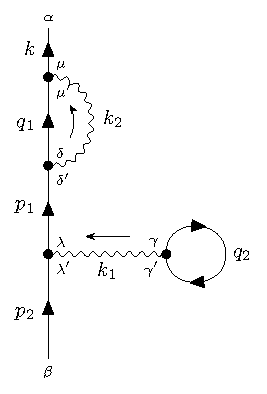
\includegraphics[width=0.5\textwidth]{images/C_label_m_2.pdf}  \label{fig:} }
\end{minipage}
\begin{minipage}[]{0.5\linewidth}
\centering
\subfloat[][After.]{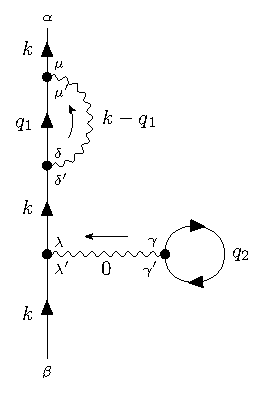
\includegraphics[width=0.5\textwidth]{images/C_label_m.pdf}  \label{fig:} }
\end{minipage}
\caption{\label{fig:2} Feynman diagram in momentum space of (\textbf{c}) before and after conservation of momenta. }
\end{figure}

Altough the topological structure is identical with the corresponding diagrams in coordinate space, the labeling and interpretation are naturally quite different.
In particular, the analitycal expression of (\textbf{c}) diagram in momentum space results:
\begin{equation*}
\begin{split}
  G_{\alpha \beta }^{(2c)} (k) &=  \frac{(-1)^1}{(2 \pi )^{8}} \qty(\frac{i}{\hbar })^2
   \sum_{\substack{\lambda \lambda', \mu \mu' \\ \gamma \gamma', \delta \delta'   } }^{}  \int_{}^{} \dd[4]{q_1} \dd[4]{q_2}   \times \\
   &
   \times G^0_{\alpha \mu } (k) U (k-q_1)_{\substack{ \mu \mu' \\ \delta \delta'} } G^0_{\mu' \delta } e^{i \omega_1 \eta } (q_1) G^0_{\delta' \lambda  } (k) U (0)_{\substack{ \lambda \lambda' \\ \gamma \gamma'} } G^0_{\lambda' \beta  } (k) G^0_{\gamma' \gamma  } (q_2) e^{i \omega_2 \eta }
\end{split}
\end{equation*}








\end{document}
